\documentclass{article}
\usepackage{tikz}
\usepackage[left=0.5cm,right=0.5cm,top=2cm,bottom=2cm]{geometry}
\begin{document}
\begin{figure}[!t]
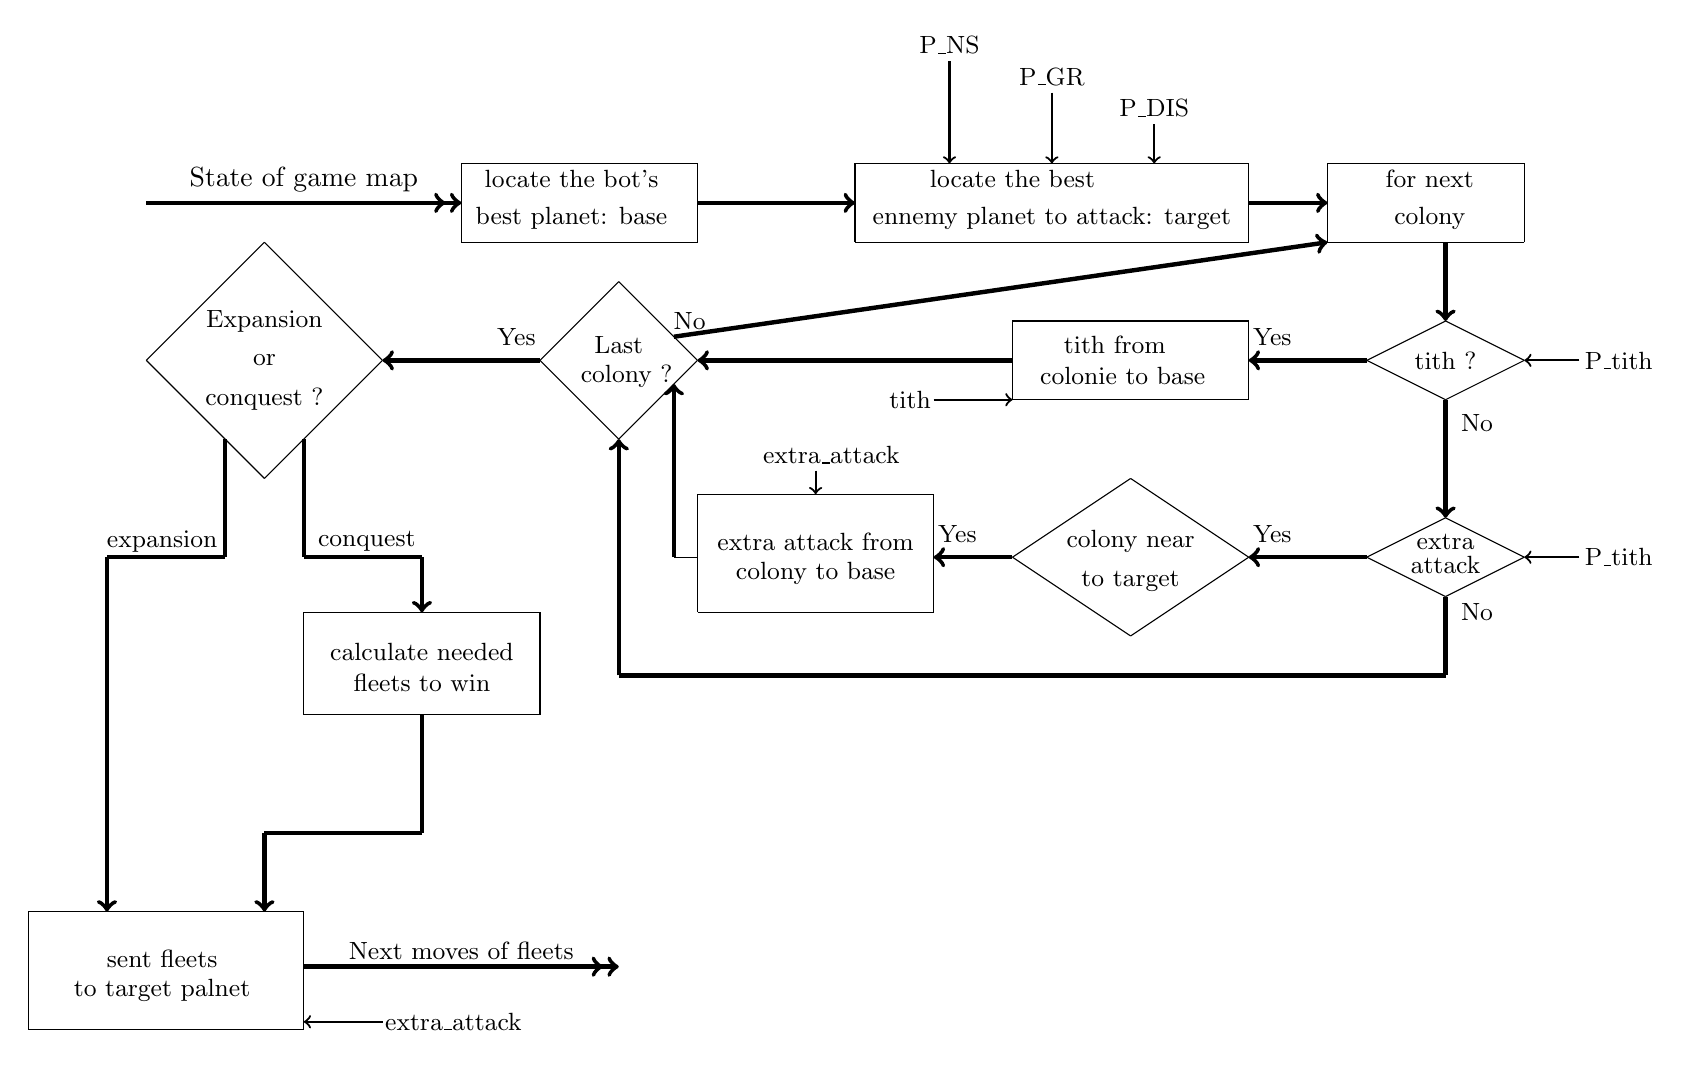
\begin{tikzpicture}
\draw [->][ultra thick](-1,20) -- (3,20);
\draw [->][ultra thick](-1,20) -- (2.8,20);
\node at (1,20.3) {State of game map};
\draw (3,20.5) --(3,19.5);
\draw (3,20.5) --(6,20.5);
\draw (6,20.5) --(6,19.5);
\draw (6,19.5) --(3,19.5);
\draw [->][ultra thick](6,20) -- (8,20);
\node at (4.4,20.3) {\small locate the bot's};
\node at (4.4,19.8) {\small best planet: base};
\draw (8,20.5) --(8,19.5);
\draw (8,20.5) --(13,20.5);
\draw (13,20.5) --(13,19.5);
\draw (13,19.5) --(8,19.5);
\draw [->][thick](9.2,21.8) -- (9.2,20.5);
\draw [->][thick](10.5,21.4) -- (10.5,20.5);
\draw [->][thick](11.8,21) -- (11.8,20.5);
\node at (10,20.3) {\small locate the best};
\node at (9.2,22) {\small P\_NS};
\node at (10.5,21.6) {\small P\_GR};
\node at (11.8,21.2) {\small P\_DIS};
\node at (10.5,19.8) {\small ennemy planet to attack: target};
\draw [->][ultra thick](13,20) -- (14,20);
\draw (14,20.5) --(14,19.5);
\draw (14,20.5) --(16.5,20.5);
\draw (16.5,20.5) --(16.5,19.5);
\draw (16.5,19.5) --(14,19.5);
\node at (15.3,20.3) {\small for next};
\node at (15.3,19.8) {\small colony};
\draw [->][ultra thick](15.5,19.5) -- (15.5,18.5);
\draw (15.5,18.5) --(14.5,18);
\draw (14.5,18) --(15.5,17.5);
\draw (15.5,17.5) --(16.5,18);
\draw (16.5,18) --(15.5,18.5);
\draw [->][thick](17.2,18) -- (16.5,18);
\node at (17.7,18) {\small P\_tith};
\draw [->][thick](17.2,15.5) -- (16.5,15.5);
\node at (17.7,15.5) {\small P\_tith};
\node at (15.5,18) {\small tith ?};
\node at (15.5,15.7) {\small extra};
\node at (15.5,15.4) {\small attack};
\draw [->][ultra thick](15.5,17.5) -- (15.5,16);
\node at (15.9,17.2) {\small No};
\draw (15.5,16) --(14.5,15.5);
\draw (14.5,15.5) --(15.5,15);
\draw (15.5,15) --(16.5,15.5);
\draw (16.5,15.5) --(15.5,16);
\draw [->][ultra thick](14.5,18) -- (13,18);
\node at (13.3,18.3) {\small Yes};
\draw [ultra thick](15.5,15) -- (15.5,14);
\node at (15.9,14.8) {\small No};
\draw [ultra thick](15.5,14) -- (5,14);
\draw [->][ultra thick](5,14) -- (5,17);
\draw (13,18.5) --(13,17.5);
\draw (13,17.5) --(10,17.5);
\draw (10,17.5) --(10,18.5);
\draw (10,18.5) --(13,18.5);
\node at (13.3,15.8) {\small Yes};
\node at (11.3,18.2) {\small tith from};
\node at (11.4,17.8) {\small colonie to base};
\node at (8.7,17.5) {\small tith};
\draw [->][thick](9,17.5) -- (10,17.5);
\draw [->][ultra thick](14.5,15.5) -- (13,15.5);
\node at (9.3,15.8) {\small Yes};
\draw (13,15.5) --(11.5,16.5);
\draw (11.5,16.5) --(10,15.5);
\draw (10,15.5) --(11.5,14.5);
\draw (11.5,14.5) --(13,15.5);
\node at (11.5,15.7) {\small colony near};
\node at (11.5,15.2) {\small to target};
\draw [->][ultra thick](10,15.5) -- (9,15.5);
\draw (9,16.3) --(9,14.8);
\draw (9,14.8) --(6,14.8);
\draw (6,14.8) --(6,16.3);
\draw (6,16.3) --(9,16.3);
\node at (7.5,15.7) {\small extra attack from};
\node at (7.5,15.3) {\small colony to base};
\draw [->][thick](7.5,16.6) -- (7.5,16.3);
\node at (7.7,16.8) {\small extra\_attack};
\draw [->][ultra thick](10,18) -- (6,18);
\draw (6,18) --(5,19);
\draw (5,19) --(4,18);
\draw (4,18) --(5,17);
\draw (5,17) --(6,18);
\node at (5,18.2) {\small Last};
\node at (5.1,17.8) {\small colony ?};
\draw [->][ultra thick](5.7,18.3) -- (14,19.5);
\node at (5.9,18.5) {\small No};
\node at (3.7,18.3) {\small Yes};
\draw (6,15.5) -- (5.7,15.5);
\draw [->][ultra thick](5.7,15.5) -- (5.7,17.7);
\draw [->][ultra thick](4,18) -- (2,18);
\draw (2,18) -- (0.5,19.5);
\draw (0.5,19.5) -- (-1,18);
\draw (-1,18) -- (0.5,16.5);
\draw (0.5,16.5) -- (2,18);
\node at (0.5,18.5) {\small Expansion };
\node at (0.5,18) {\small or };
\node at (0.5,17.5) {\small conquest ?};
\draw [ultra thick](1,17) -- (1,15.5);
\draw [ultra thick](1,15.5) -- (2.5,15.5);
\node at (1.8,15.7) {\small conquest};
\draw [->][ultra thick](2.5,15.5) -- (2.5,14.8);
\draw (1,14.8) -- (4,14.8);
\draw (4,14.8) -- (4,13.5);
\draw (4,13.5) -- (1,13.5);
\draw (1,13.5) -- (1,14.8);
\node at (2.5,14.3) {\small calculate needed};
\node at (2.5,13.9) {\small fleets to win};
\draw [ultra thick](0,17) -- (0,15.5);
\draw [ultra thick](0,15.5) -- (-1.5,15.5);
\draw [->][ultra thick](-1.5,15.5) -- (-1.5,11);
\draw (-2.5,11) -- (1,11);
\draw (-2.5,9.5) -- (1,9.5);
\draw (-2.5,11) -- (-2.5,9.5);
\draw (1,11) -- (1,9.5);
\draw [ultra thick](2.5,13.5) -- (2.5,12);
\draw [ultra thick](2.5,12) -- (0.5,12);
\node at (-0.8,15.7) {\small expansion};
\draw [->][ultra thick](0.5,12) -- (0.5,11);
\node at (-0.8,10.4) {\small sent fleets};
\node at (-0.8,10) {\small to target palnet};
\draw [->][ultra thick](1,10.3) -- (4.8,10.3);
\draw [->][ultra thick](1,10.3) -- (5,10.3);
\node at (3,10.5) {\small Next moves of fleets};
\draw [->][thick](2,9.6) -- (1,9.6);
\node at (2.9,9.6) {\small extra\_attack};
\end{tikzpicture}
\end{figure}
\end{document}